\chapter{Introducción}
\label{sec:intro}
\pagenumbering{arabic} % para empezar la numeración de página con números

El despliegue de redes IoT (Internet de las Cosas) representa la piedra angular en la transición de las urbes tradicionales hacia las \textit{Smart Cities} (o Ciudades Inteligentes). Históricamente, la planificación urbana y la gestión del tráfico se basaban en estudios estadísticos puntuales que quedaban obsoletos rápidamente. Sin embargo, la integración del IoT ha transformado la infraestructura física de las ciudades en un ecosistema digital dinámico e interconectado.

En este nuevo paradigma, los sensores IoT actúan como el ``sistema nervioso'' de la ciudad. Estos dispositivos, integrados en el asfalto, semáforos, farolas o contenedores, son capaces de capturar, procesar y transmitir parámetros físicos en tiempo real. La verdadera disrupción tecnológica del IoT urbano no reside únicamente en la recolección aislada de datos, sino en la capacidad de generar un flujo continuo de información a gran escala (\textit{Big Data}). Esto permite a las administraciones públicas y a los sistemas automatizados pasar de una gobernanza reactiva, que actúa cuando el problema ya se ha manifestado, a una proactiva y predictiva, lo que permite maximizar la eficiencia y anticipar casuísticas de interés.

\subsection{Motivación}
\label{subsec:motivacion}
El impacto del IoT en la movilidad urbana es especialmente crítico. En las últimas décadas, el crecimiento demográfico y la rápida urbanización han transformado la congestión vehicular en uno de los mayores desafíos para las administraciones públicas, generando un impacto negativo tanto en el medio ambiente, por el aumento de emisiones de gases de efecto invernadero, como en la calidad de vida de los ciudadanos. Diversos estudios urbanísticos señalan que el tráfico de agitación ---aquel provocado por vehículos que circulan a baja velocidad buscando activamente aparcamiento--- es responsable de hasta un 30\% de la congestión en los centros urbanos, lo que representa una fuente masiva de contaminación atmosférica y acústica~\cite{shoup2006cruising}.

Para mitigar este problema, la instalación de sensores electromagnéticos o de infrarrojos en las plazas de aparcamiento en superficie permite monitorizar la ocupación exacta en tiempo real. No obstante, la implementación práctica de estas redes de sensores se enfrenta a un desafío técnico ineludible: la volatilidad y la pérdida de integridad de los datos. Al tratarse de dispositivos físicos distribuidos en un entorno hostil (la vía pública), los sensores están sujetos a fallos de conectividad, latencia de red, averías por factores climáticos o agotamiento de baterías~\cite{algaradi2020survey}. Consecuentemente, las series temporales de datos quedan discontinuas y plagadas de valores faltantes, lo que distorsiona severamente cualquier análisis visual o intento de toma de decisiones informada.

Por consiguiente, la motivación principal de este proyecto surge de la necesidad de construir un ecosistema integral y resiliente que aborde el ciclo de vida completo del dato urbano. No es suficiente con instalar sensores; es imperativo diseñar una arquitectura de ingeniería de datos robusta y automatizada que ingeste y almacene esta información en tiempo real. Asimismo, es crucial la aplicación de técnicas vanguardistas de \textit{Deep Learning} capaces de comprender los patrones espaciotemporales subyacentes para imputar y reconstruir la información faltante cuando el hardware falla. Solo garantizando esta calidad e integridad técnica, el flujo incesante de datos del IoT puede ser explotado eficazmente, transformando los datos crudos en valor real y democratizado para la ciudadanía.

\subsection{Caso de Estudio: La ciudad de Melbourne}
\label{subsec:caso_estudio}

Para materializar y validar la arquitectura propuesta, este proyecto toma como escenario de aplicación la red de aparcamientos en superficie de la ciudad de Melbourne (Australia). La elección de esta urbe responde a criterios técnicos y de disponibilidad de datos que la convierten en un entorno de pruebas óptimo para el desarrollo del proyecto.

En primer lugar, el gobierno local de Melbourne es pionero a nivel mundial en políticas de \textit{Open Data}, al ofrecer acceso público y documentado a su infraestructura IoT. A diferencia de otras grandes ciudades que únicamente proporcionan datos agregados de aparcamientos subterráneos, Melbourne ofrece una granularidad a nivel de plaza individual.

En segundo lugar, la plataforma proporciona una dualidad de acceso crítica para este proyecto. Por un lado, un repositorio histórico masivo, como el \textit{dataset} del año 2019 escogido para este proyecto, el cual es indispensable para la fase de entrenamiento de modelos de \textit{Deep Learning}. Por otro lado, una API REST que emite el estado de los sensores en tiempo real, lo cual habilita la implementación de un \textit{pipeline} de orquestación continua.

Finalmente, al tratarse de una red de sensores físicos expuesta a condiciones urbanas reales durante años, el conjunto de datos de Melbourne no es un entorno estéril o simulado. Contiene intrínsecamente las imperfecciones, latencias, fallos de batería y valores faltantes descritos en la motivación de este trabajo. Esta naturaleza imperfecta es precisamente lo que legitima y hace necesaria la aplicación de herramientas de imputación avanzadas como PyPOTS, lo que permite demostrar el valor de la solución propuesta en un escenario de extrema fidelidad con el mundo real.

\section{Estado del Arte}
\label{sec:estado_arte}

\subsection{Consolidación del IoT en la Gestión Inteligente del Aparcamiento}
\label{subsec:estado_iot}

En la última década, el Internet de las Cosas (IoT) ha superado su fase experimental para consolidarse como la infraestructura subyacente de las \textit{Smart Cities}. Este avance ha sido impulsado por el despliegue de redes de bajo consumo y largo alcance (LPWAN) y la transición hacia el \textit{Edge Computing}, lo cual hace posible sensorizar masivamente infraestructuras críticas urbanas~\cite{alavi2018internet}.

Dentro de la movilidad urbana, el \textit{Smart Parking} destaca como uno de los campos con mayor madurez tecnológica. La información generada por los sensores ha dejado de ser puramente descriptiva para integrarse en tres grandes casos de uso operativos: (I) sistemas de guiado en tiempo real para reducir el tráfico de agitación; (II) tarificación dinámica (\textit{Dynamic Pricing}) basada en la demanda espacial; y (III) control telemático de infracciones (\textit{Enforcement}). Sin embargo, el verdadero potencial de estos sistemas requiere trascender la monitorización actual hacia la analítica predictiva, lo cual exige infraestructuras de procesamiento de datos altamente eficientes~\cite{lin2017survey}.

\subsection{Evolución hacia el \textit{Modern Data Stack} en Entornos IoT}
\label{subsec:estado_data_stack}

El procesamiento del ingente volumen de datos espaciotemporales generado por las redes ha evidenciado las limitaciones de las arquitecturas monolíticas tradicionales ETL (\textit{Extract, Transform, Load}). Históricamente, la gestión de estos flujos requería bases de datos pesadas y costosos clústeres computacionales.

Actualmente, el estado del arte a nivel industrial y de investigación converge hacia el paradigma del \textit{Modern Data Stack} (MDS). Esta evolución se caracteriza por la adopción de herramientas ágiles, desacopladas y orientadas al código (\textit{Data-as-Code}). En la fase de orquestación, planificadores dinámicos como Apache Airflow se han estandarizado para gestionar dependencias complejas de ingesta. Simultáneamente, el paradigma de almacenamiento analítico ha experimentado una disrupción con la aparición de motores OLAP (procesamiento analítico en línea) en proceso (\textit{in-process}), entre los que DuckDB destaca como su máximo exponente actual. Estos sistemas permiten ejecutar consultas vectorizadas sobre datos IoT directamente en entornos locales o \textit{edge}, superando la latencia inherente a las bases de datos cliente-servidor tradicionales~\cite{raasveldt2019duckdb}.

\subsection{Modelado de Series Temporales y el Reto de los Datos Parcialmente Observados}
\label{subsec:estado_imputacion}

Pese a contar con infraestructuras de datos robustas, la extracción de valor predictivo se topa con el desafío técnico expuesto en la motivación: la naturaleza intermitente de la señal física. Los algoritmos clásicos de \textit{Machine Learning} y las redes neuronales estándar tienen un comportamiento errático ante la presencia de huecos o valores nulos en las secuencias temporales.

En los últimos años, el análisis secuencial ha dado un salto cualitativo gracias a la adaptación de arquitecturas de \textit{Deep Learning} avanzadas (\textit{Transformers}) al dominio temporal. No obstante, la vanguardia investigadora actual no se centra únicamente en la predicción pura, sino en el modelado de Datos Temporales Parcialmente Observados (\textit{Partially Observed Time Series} o POTS).

Para abordar esta problemática, la comunidad científica ha transitado desde heurísticas simples hacia \textit{frameworks} de aprendizaje profundo especializados en imputación. Librerías recientes de código abierto, como PyPOTS, se han posicionado como el estándar en investigación~\cite{du2023pypots}. Estas herramientas implementan modelos capaces de inferir el dato faltante basándose en el contexto espacio-temporal global de la serie, para así alimentar los posteriores cuadros de mando analíticos y sistemas de información geográfica con información íntegra y fiable.

\section{Objetivos del proyecto}
\label{sec:objetivos}

\subsection{Objetivo general}
\label{subsec:obj_general}

Desarrollar un sistema integral de procesamiento y modelado para predecir la disponibilidad de plazas de aparcamiento en superficie, gestionando y reconstruyendo series temporales espacialmente distribuidas provenientes de una red de datos de sensores IoT en tiempo real.

\subsection{Objetivos específicos}
\label{subsec:obj_especificos}

Para alcanzar el objetivo general, el proyecto se desglosa en las siguientes metas técnicas secuenciales:

\begin{itemize}
	\item \textbf{Realizar un Análisis Exploratorio de Datos históricos (EDA).} Analizar el conjunto de datos históricos masivos para identificar distribuciones, patrones de estacionalidad en la movilidad urbana y anomalías en los tiempos de estacionamiento.
	
	\item \textbf{Preprocesar el \textit{dataset} y entrenar el modelo.} Acondicionar el conjunto de datos y posteriormente entrenar el modelo de PyPOTS, para que el algoritmo aprenda los patrones subyacentes de ocupación y la estructura de la serie temporal.
	
	\item \textbf{Desplegar la infraestructura de ingesta y almacenamiento continuo.} Orquestar un \textit{pipeline} automatizado utilizando Apache Airflow para consumir datos en tiempo real de la API de Melbourne durante un periodo ininterrumpido de un mes, y almacenar el histórico resultante en una base de datos analítica centralizada (DuckDB).
	
	\item \textbf{Imputar datos faltantes en la serie temporal actual.} Aplicar el modelo PyPOTS previamente entrenado sobre los datos reales recopilados durante el mes de monitorización con Airflow, con el fin de reconstruir la serie temporal e imputar los valores faltantes (\textit{missing data}) generados por los fallos inherentes de la sensórica física.
	
	\item \textbf{Desarrollar un \textit{dashboard} analítico.} Construir un cuadro de mando interactivo conectando Grafana directamente a DuckDB para la monitorización de datos y métricas. 
	
	\item \textbf{Construir un visualizador geoespacial.} Visualizar la red de aparcamientos categorizada por su proximidad a Puntos de Interés (POIs) en un mapa 2D.
	
	\item \textbf{Divulgar los resultados mediante un entorno web estructurado.} Diseñar y desplegar una página web interactiva con Quarto, dividida en tres secciones principales, que actúe como portfolio visual para exponer la metodología, la arquitectura de datos y los resultados del proyecto de manera accesible.
\end{itemize}

\section{Planificación temporal}
\label{sec:planificacion}

Para garantizar la consecución de los objetivos descritos y asegurar la viabilidad técnica, el ciclo de vida del proyecto se ha estructurado en cuatro fases de desarrollo iterativo e incremental. 

\begin{itemize}
	\item \textbf{Fase 1: Conceptualización y despliegue de infraestructura.} En esta etapa inicial se llevó a cabo la revisión bibliográfica del estado del arte y el diseño teórico de la arquitectura. Seguidamente, se configuraron los entornos virtualizados y se implementaron los flujos de orquestación con Apache Airflow, y se estableció la conexión temprana con la API de Melbourne para posteriormente iniciar la ventana de ingesta y almacenamiento continuo en DuckDB.
	
	\item \textbf{Fase 2: Procesamiento histórico y \textit{Feature Engineering}.} Esta fase se centró en la adecuación del conjunto de datos masivo correspondiente al año 2019. Se ejecutaron labores de limpieza, integración de metadatos geoespaciales y, fundamentalmente, el remuestreo (\textit{resampling}) de los eventos vehiculares asíncronos. Esto permitió estandarizar la información y construir las matrices temporales con valores nulos explícitos requeridas para el modelado.
	
	\item \textbf{Fase 3: Modelado predictivo y visualizaciones.} Con los datos estructurados, se procedió al diseño, entrenamiento y ajuste de los modelos de \textit{Deep Learning} de PyPOTS. En paralelo, se construyó el ecosistema de visualización conectando Grafana a la base de datos analítica y desarrollando mapas interactivos para la representación espacial de las plazas y su relación con lugares próximos relevantes.
	
	\item \textbf{Fase 4: Validación y Cierre.} La etapa final consistió en la validación del ecosistema, aplicando el modelo entrenado sobre los datos recopilados en tiempo real para ejecutar la imputación de valores faltantes. Finalmente, se desplegó el entorno web divulgativo mediante Quarto y se procedió a la extracción de conclusiones y revisión exhaustiva de la presente memoria académica.
\end{itemize}

El proyecto se ha desarrollado durante el periodo comprendido entre los meses de enero y junio. El avance técnico se ha abordado mediante una metodología de trabajo continua, integrando la ejecución práctica de las fases descritas con la redacción y revisión progresiva de la presente memoria académica.

\subsection{Diagrama de Gantt}
\label{subsec:gantt}

Para ilustrar visualmente la planificación temporal detallada en la sección anterior, se ha elaborado el diagrama de Gantt correspondiente al ciclo de vida del proyecto. Esta representación gráfica permite observar la duración y secuenciación de las tareas específicas que componen cada una de las cuatro fases principales.

\begin{figure}[htbp]
	\centering
	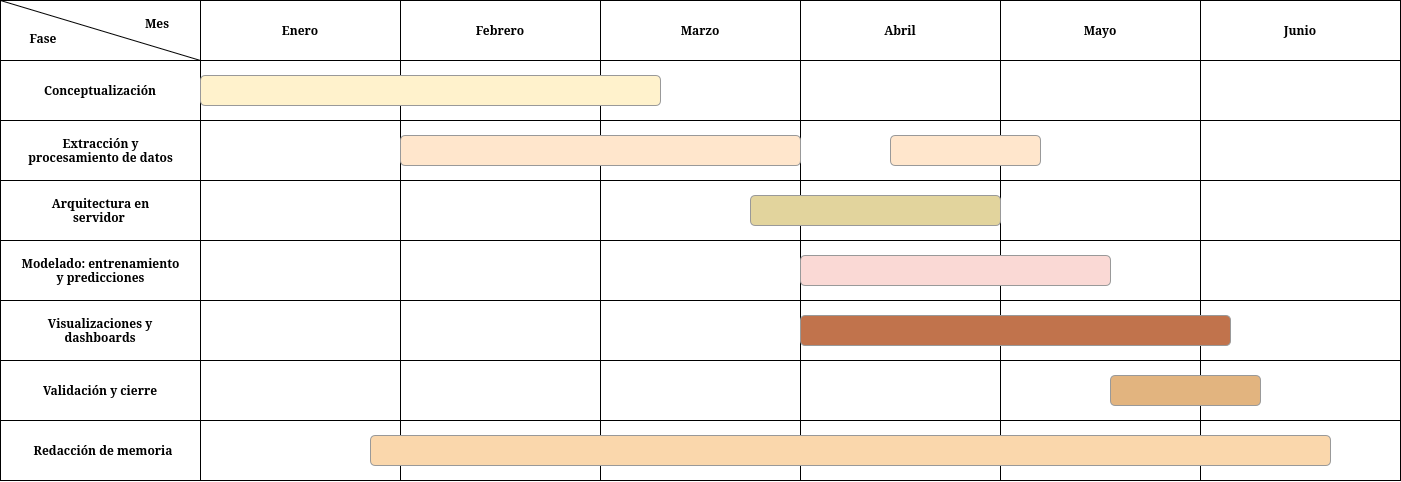
\includegraphics[width=15cm, keepaspectratio]{img/[implem]diagrama_gantt.png}
	\caption{Diagrama de Gantt ilustrando la temporalización de las fases del proyecto y sus respectivas tareas a lo largo de seis meses.}
	\label{fig:diagrama_gantt}
\end{figure}



\section{Estructura de la memoria}
\label{sec:estructura}

El resto del presente documento se estructura en cuatro capítulos adicionales, organizados de manera secuencial para reflejar el ciclo de vida del proyecto:

\begin{itemize}
	\item El \textbf{capítulo~\ref{chap:tecnologias}} (Tecnologías empleadas) detalla las herramientas, lenguajes y \textit{frameworks} utilizados para la consecución del proyecto. Se justifica la elección de cada pieza de \textit{software} dentro del paradigma del \textit{Modern Data Stack}.
	
	\item El \textbf{capítulo~\ref{chap:diseño}} (Diseño e Implementación) constituye el núcleo técnico de la memoria. En él se describe exhaustivamente el desarrollo del \textit{pipeline} de datos, los procesos de limpieza y \textit{resampling} del conjunto histórico, así como el entrenamiento del modelo de predicción. Asimismo, se detallan el diseño arquitectónico de la orquestación en tiempo real y la construcción del ecosistema de visualización analítica y geoespacial.
	
	\item El \textbf{capítulo~\ref{chap:experimentos}} (Experimentación y Resultados) presenta las pruebas realizadas y los hallazgos obtenidos. Se evalúa el rendimiento del modelo de imputación espacial y temporal entrenado con los datos reales recopilados durante la ventana de monitorización, y se exponen los resultados visuales de los dashboard.
	
	\item Finalmente, el \textbf{capítulo~\ref{chap:conclusiones}} (Conclusiones) sintetiza las deducciones finales extraídas tras la finalización del trabajo. Posteriormente, se evalúa el grado de cumplimiento de los objetivos planteados y se proponen futuras líneas de investigación y desarrollo que podrían derivarse de esta base.
\end{itemize}